%% LaTeX2e class for student theses
%% sections/content.tex
%% 
%% Karlsruhe Institute of Technology
%% Institute for Program Structures and Data Organization
%% Chair for Software Design and Quality (SDQ)
%%
%% Dr.-Ing. Erik Burger
%% burger@kit.edu
%%
%% Version 1.3.6, 2022-09-28

\chapter{Introduction}
\label{ch:Introduction}

%% -------------------
%% | Example content |
%% -------------------

% This is the SDQ thesis template.
% For more information on the formatting of theses at SDQ, please refer to
% \url{https://sdq.kastel.kit.edu/wiki/Ausarbeitungshinweise} or to your advisor.

% \section{Spacing and indentation}
% To separate parts of text in \LaTeX, please use two line breaks.
% They will then be set with correct indentation.
% Do \emph{not} use:
% \begin{itemize}
%   \itemsep0em
%   \item \texttt{\textbackslash\textbackslash}
%   \item \texttt{\textbackslash parskip}
%   \item \texttt{\textbackslash vskip}
% \end{itemize} 
% or other commands to manually insert spaces, since they break the layout of this template.

% \section{Example: Citation}
% \label{sec:Introduction:Citation}
% This template is based on \texttt{biblatex} and \texttt{biber}, which is preferred over the
% outdated Bib\TeX{} software.
% Please adjust your build environment if necessary (see
% \url{https://sdq.kastel.kit.edu/wiki/BibTeX-Literaturlisten#biblatex.2Fbiber})

% A citation: \cite{becker2008a} 

% \section{Example: Figures}
% \label{sec:Introduction:Figures}
% \begin{figure}
% \centering
% 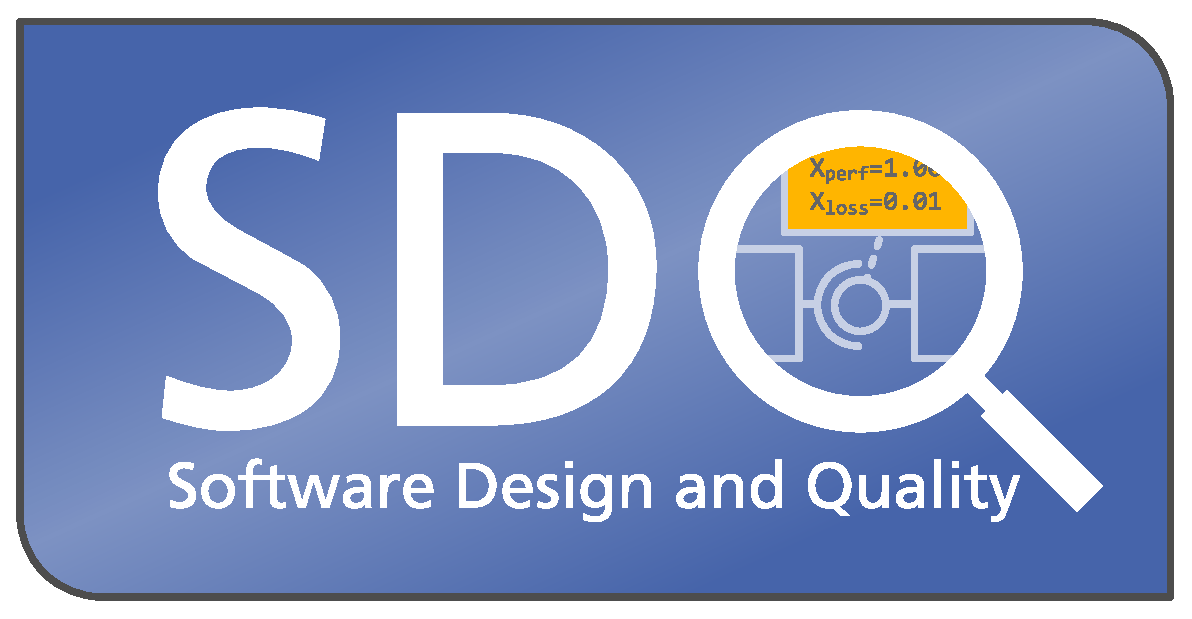
\includegraphics[width=4cm]{logos/sdqlogo}
% \caption{SDQ logo}
% \label{fig:sdqlogo}
% \end{figure}

% A reference: The SDQ logo is displayed in \autoref{fig:sdqlogo}. 
% (Use \code{\textbackslash autoref\{\}} for easy referencing.) 

% \section{Example: Tables}
% The \texttt{booktabs} package offers nicely typeset tables, as in \autoref{tab:atable}.

% \label{sec:Introduction:Tables}
% \begin{table}
% \centering
% \begin{tabular}{r l}
% \toprule
% abc & def\\
% ghi & jkl\\
% \midrule
% 123 & 456\\
% 789 & 0AB\\
% \bottomrule
% \end{tabular}
% \caption{A table}
% \label{tab:atable}
% \end{table}

% \section{Example: Formula}
% One of the nice things about the Linux Libertine font is that it comes with
% a math mode package.
% \begin{displaymath}
% f(x)=\Omega(g(x))\ (x\rightarrow\infty)\;\Leftrightarrow\;
% \limsup_{x \to \infty} \left|\frac{f(x)}{g(x)}\right|> 0
% \end{displaymath}

%% --------------------
%% | /Example content |
%% --------------------

Research in Machine Learning and especially Deep Learning has produced an abundance of highly influential work in recent years, like
Convolutional Neural Networks (CNNs), Transformers and Generative Adversarial Networks (GANs). These Machine Learning Models are
becoming ever more accurate, achieving or even surpassing human-level performance on tasks like visual perception or natural language
understanding. Because of their high potential for innovation, Machine Learning Models are increasingly being used in real-world 
applications. To profit from this, a multitude of technology enterprises offer numerous services to ease the training, development and
deployment of Machine Learning applications. These services can be grouped together under the term Machine Learning as a Service (MLaaS). \\
While MLaaS is crucial to make Machine Learning more accessable, it also poses a security threat. In the past years, numerous research works
have been published which demonstrate how easily Machine Learning Models can be extracted from MLaaS services \cite{tramer2016stealing}
\cite{reith2019efficiently} \cite{papernot2017practical}. The standard procedure to steal a such a machine learning model is to train a local
clone (also called substitute model) of the model which is hosted on the MLaaS service (also called target model). The substitute model is trained
using a dataset that the attacker collects which is also called thief dataset. Labels for the thief dataset are then obtained by querying the target
model on the thief dataset. The process of extracting Machine Learning models from MLaaS services is referred to as Model Stealing. \\
Because of the dramatic consequences of Model Stealing Attacks, researchers have also investigated how to defend against them. Two recent approaches
to defend Model Stealing Attacks are Prediction Poisoning \cite{orekondy2019prediction} and PRADA \cite{juuti2019prada}. Despite the effort to
defend model stealing attacks, research works have been published which evade these defense strategies. One notable example of this is the model
extraction framework ActiveThief \cite{pal2020activethief} which successfully evades the PRADA defense strategy. ActiveThief makes use of Active
Learning to determine which samples of the thief dataset it should query the target model on. Active Learning is an intensively studied research
field which aims to minimize the labeling effort in the training process of Machine Learning models. The problem of Active Learning is however that it
needs a lot of computing resources. In this work, we extend on the ActiveThief framework by using \textit{Continual} Active Learning in the model
extraction process.\par
Continual Learning is a research field which aims to make Machine Learning Models more robust against the introduction of new data. The major problem
of the classic training procedure is that a model trained on a new task rapidly loses the ability to perform any previous tasks it was trained on.
Research in Continual Learning aims to develop methods which allow Machine Learning Models to learn new tasks without forgetting the knowledge of old 
tasks. \par
\textbf{Contributions} \hspace{0.2cm} The objective of this thesis is to combine existing approaches of the continual learning domain
 with approaches in the active learning domain. More specifically, we are focusing on regularization-based continual learning methods
whereas we use both uncertainty-based and diversity-based active learning methods. The continual learning methods we use are Elastic
Weight Consolidation (EWC) \cite{kirkpatrick2017overcoming}, Memory Aware Synapses (MAS) \cite{aljundi2018memory}, Incremental Moment Matching
(IMM) \cite{lee2017overcoming} and Asymmetric Loss Approximation by Single-Side Overestimation (ALASSO) \cite{park2019continual}.
Concerning active learning, we compare random sampling, Least Confidence (LC) \cite{lewis1994sequential} sampling, Batch Active Learning by
Diverse, uncertain Gradient lower Bound (BADGE) \cite{ash2019deep}, Bayesian Active Learning by Disagreement (BALD) \cite{houlsby2011bayesian} and
CoreSet \cite{sener2017active}.
We analyze how the continual learning methods can speed up the active learning process, which combinations of continual and active learning methods
are most effective and how the trade-off between accuracy and speed up is. While the focus of this thesis is on regularization-based continual
learning methods, we briefly explore the effectiveness of exemplar rehearsal continual learning using the Average Gradient Episodic Memory (AGEM)
approach \cite{chaudhry2018efficient} combined with representation-based active learning in form of Variational Adversarial Active Learning (VAAL)
\cite{sinha2019variational}. \par
After exploring the effectiveness of the different combinations of continual and active learning methods, we apply these combinations in the model stealing
domain. More specifically, we build upon the model extraction framework ActiveThief \cite{pal2020activethief} and investigate the performance of continual
active learning methods in the model stealing domain.
